\documentclass{article}[18pt]
\ProvidesPackage{format}
%Page setup
\usepackage[utf8]{inputenc}
\usepackage[margin=0.7in]{geometry}
\usepackage{parselines} 
\usepackage[english]{babel}
\usepackage{fancyhdr}
\usepackage{titlesec}
\hyphenpenalty=10000

\pagestyle{fancy}
\fancyhf{}
\rhead{Sam Robbins}
\rfoot{Page \thepage}

%Characters
\usepackage{amsmath}
\usepackage{amssymb}
\usepackage{gensymb}
\newcommand{\R}{\mathbb{R}}

%Diagrams
\usepackage{pgfplots}
\usepackage{graphicx}
\usepackage{tabularx}
\usepackage{relsize}
\pgfplotsset{width=10cm,compat=1.9}
\usepackage{float}

%Length Setting
\titlespacing\section{0pt}{14pt plus 4pt minus 2pt}{0pt plus 2pt minus 2pt}
\newlength\tindent
\setlength{\tindent}{\parindent}
\setlength{\parindent}{0pt}
\renewcommand{\indent}{\hspace*{\tindent}}

%Programming Font
\usepackage{courier}
\usepackage{listings}
\usepackage{pxfonts}

%Lists
\usepackage{enumerate}
\usepackage{enumitem}

% Networks Macro
\usepackage{tikz}


% Commands for files converted using pandoc
\providecommand{\tightlist}{%
	\setlength{\itemsep}{0pt}\setlength{\parskip}{0pt}}
\usepackage{hyperref}

% Get nice commands for floor and ceil
\usepackage{mathtools}
\DeclarePairedDelimiter{\ceil}{\lceil}{\rceil}
\DeclarePairedDelimiter{\floor}{\lfloor}{\rfloor}

% Allow itemize to go up to 20 levels deep (just change the number if you need more you madman)
\usepackage{enumitem}
\setlistdepth{20}
\renewlist{itemize}{itemize}{20}

% initially, use dots for all levels
\setlist[itemize]{label=$\cdot$}

% customize the first 3 levels
\setlist[itemize,1]{label=\textbullet}
\setlist[itemize,2]{label=--}
\setlist[itemize,3]{label=*}

% Definition and Important Stuff
% Important stuff
\usepackage[framemethod=TikZ]{mdframed}

\newcounter{theo}[section]\setcounter{theo}{0}
\renewcommand{\thetheo}{\arabic{section}.\arabic{theo}}
\newenvironment{important}[1][]{%
	\refstepcounter{theo}%
	\ifstrempty{#1}%
	{\mdfsetup{%
			frametitle={%
				\tikz[baseline=(current bounding box.east),outer sep=0pt]
				\node[anchor=east,rectangle,fill=red!50]
				{\strut Important};}}
	}%
	{\mdfsetup{%
			frametitle={%
				\tikz[baseline=(current bounding box.east),outer sep=0pt]
				\node[anchor=east,rectangle,fill=red!50]
				{\strut Important:~#1};}}%
	}%
	\mdfsetup{innertopmargin=10pt,linecolor=red!50,%
		linewidth=2pt,topline=true,%
		frametitleaboveskip=\dimexpr-\ht\strutbox\relax
	}
	\begin{mdframed}[]\relax%
		\centering
		}{\end{mdframed}}



\newcounter{lem}[section]\setcounter{lem}{0}
\renewcommand{\thelem}{\arabic{section}.\arabic{lem}}
\newenvironment{defin}[1][]{%
	\refstepcounter{lem}%
	\ifstrempty{#1}%
	{\mdfsetup{%
			frametitle={%
				\tikz[baseline=(current bounding box.east),outer sep=0pt]
				\node[anchor=east,rectangle,fill=blue!20]
				{\strut Definition};}}
	}%
	{\mdfsetup{%
			frametitle={%
				\tikz[baseline=(current bounding box.east),outer sep=0pt]
				\node[anchor=east,rectangle,fill=blue!20]
				{\strut Definition:~#1};}}%
	}%
	\mdfsetup{innertopmargin=10pt,linecolor=blue!20,%
		linewidth=2pt,topline=true,%
		frametitleaboveskip=\dimexpr-\ht\strutbox\relax
	}
	\begin{mdframed}[]\relax%
		\centering
		}{\end{mdframed}}
\lhead{Software Methodlogies - Machine Learning}


\begin{document}
\begin{center}
\underline{\huge Generalisation, Training and Test Set Representation}
\end{center}
\section{Generalisation}
\begin{center}
	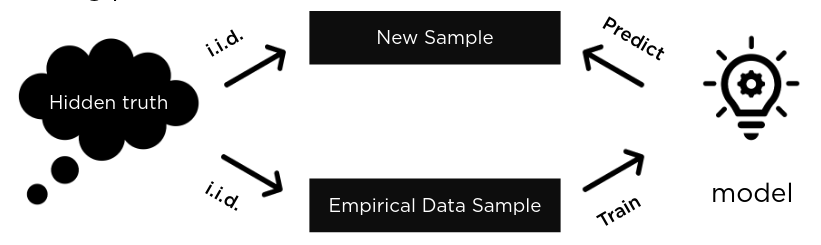
\includegraphics[scale=0.7]{Generalisation}
\end{center}
\begin{itemize}
	\item Goal - to predict well on new data drawn from (hidden) true distribution
	\item Issue - we don't see the truth, but we only get to sample from it
	\item If it fits current sample well, how can we trust it will predict well on other new samples?
\end{itemize}
How do we know if our model is good?
\begin{itemize}
	\item Theoretically
	\begin{itemize}
		\item Generalisation theory - based on ideas of measuring model simplicity/complexity
	\end{itemize}
	\item Intuition: formalisation of Ockham's razor principle
	\begin{itemize}
		\item The less complex a model is, the more likely a good empirical result is
	\end{itemize}
	\item Empirically
	\begin{itemize}
		\item Asking: will our model do well on a new sample of data 
		\item Evaluate: get a new sample of data - call it the set set
		\item Good performance on the test set is a useful indicator of good performance
	\end{itemize}
\end{itemize}
Three basic assumptions in all of the above
\begin{enumerate}
	\item We draw examples independently and identically at random from the distribution
	\item The distribution is stationary - it doesn't change over time
	\item We always pull from the same distribution, including training, validation and test sets
\end{enumerate}
\section{Training and Test set}
\textbf{Larger Training Set} - The better model we will be able to learn\\
\textbf{Larger Test Set} - The better we will be able to have confidence in evaluation metrics and tighter confidence intervals\\
\\
Ensure the test set meets the following 2 conditions:
\begin{itemize}
	\item Is large enough to yield statistically meaningful results
	\item Is representative of the data set as a whole
\end{itemize}
\subsection{Validation Set}
\begin{center}
	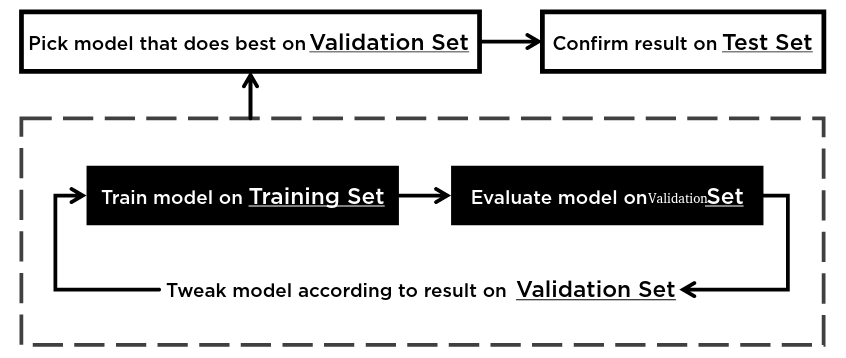
\includegraphics[scale=0.7]{Validation}
\end{center}
\begin{enumerate}
	\item Keeping the test data way off to the side (completely unused)
	\item Pick the model that does best on the validation set
	\item Double check that model against the test set 
\end{enumerate}
This is a better workflow because it creates fewer exposures to the test set
\section{Representation}
We must create a representation of the data to provide the model with a useful vantage point into the data's key qualities. That is, in order to train a model, we must choose the set of features that best represent the data
\subsection{Numeric}
This works for some models, but in some cases the gradient will change throughout, so would not work
\subsection{Bucketing}
One categorical feature is created for each bucket (sections). Then a fitting can be created for each bucket
\subsection{Categorical}
\textbf{One hot encoding} - Only one category selected at a time (e.g. a person can only have one blood type)\\
\\
If there are a small number of categories, then use the raw value, for larger numbers, hashing may be needed.
\subsection{Feature Crossing}
Two different features (e.g. age and blood type), then connect together as one feature (e.g. young people with blood type A)
\subsection{Hashing}
\begin{itemize}
	\item Save memory and time
	\item Adds some noise, but limits the maximum number of possibilities
\end{itemize}
\subsection{Embedding}
\begin{itemize}
	\item Powerful ways to represent large vocabularies
	\item Tell the model that objects with different names mean the same thing (group together)
	\item For example rabbit and bunny could be grouped together
\end{itemize}









\end{document}